\subsection{Sprint 10: da 2024-07-22 a 2024-08-04}
\par Durante lo sprint, il gruppo si occuperà di verificare gli ultimi documenti da rilasciare e, in seguito, di avviare la progettazione architetturale del software.

\subsubsection{Obiettivi}
\begin{itemize}
  \item Aggiornamento delle convenzioni per lo stile di codifica nelle \NdP;
  \item Verifica e rilascio dei seguenti documenti:
  \begin{itemize}
    \item \NdP;
    \item \PdP;
    \item \AdR{} (post colloquio \RTB);
    \item \PdQ.
  \end{itemize}
  \item Avvio della progettazione architetturale;
  \item Individuazione di stili e pattern architetturali per il back-end e il front-end;
  \item Prima stesura del documento di \ST{}.
\end{itemize}

\begin{figure}[H]
  \centering
  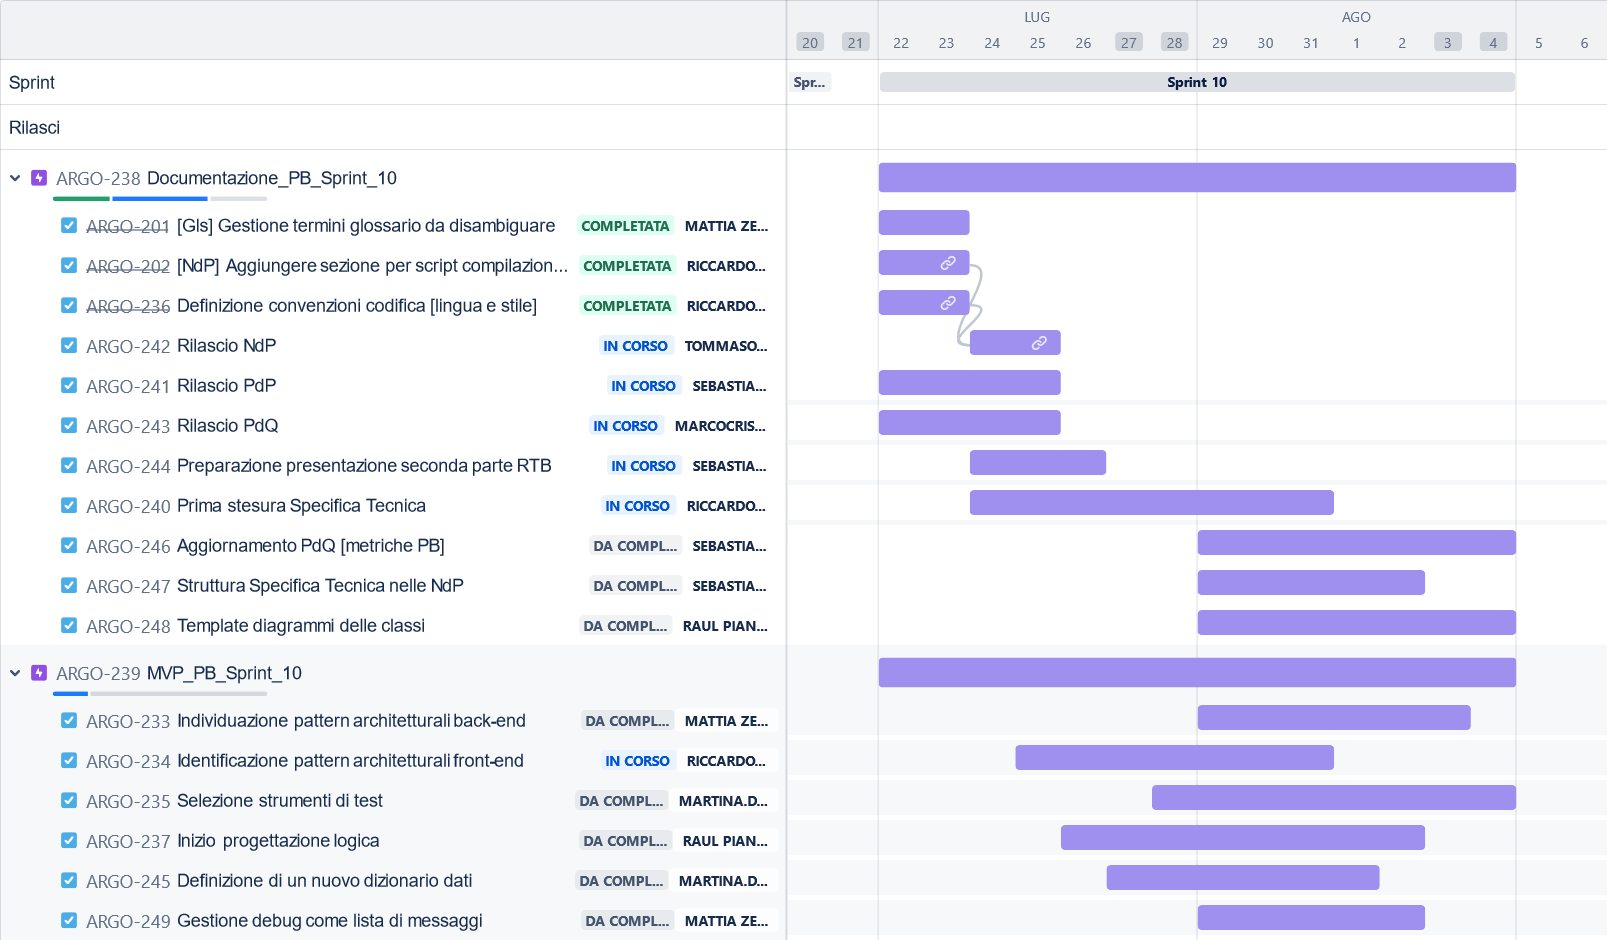
\includegraphics[width=0.90\textwidth]{assets/Pianificazione/Sprint-10/gantt.png}
  \caption{Sprint 10 - Diagramma di Gantt}\label{fig:sprint-10-gantt}
\end{figure}

